\subsection{sCenario and gOal based SysteM develOpment methoD (COSMOD) (FDD)}\label{scgo}
COSMOD-Requirements Engineering (COSMOD-RE) beschreibt ein iteratives Vorgehen zum gleichzeitigen Design von Anforderungen und Software-Architektur. Kerngedanke bei COSMOD-RE ist eine Aufteilung in vier Hierarchiestufen, wo sowohl Architektur als auch Anforderungen definiert werden. In diesen vier Hierarchiestufen wird einerseits aus der Anforderungssicht und andererseits aus der Architektursicht betrachtet, welche Anforderungen und Komponenten dem System zuzuordnen sind.\\

\subsubsection{Ziele der Methode}
Kernziel von COSMOD-RE ist es die Entwicklung von Anforderungs- und Architekturartefakten für softwareintensive eingebettete Systeme zu unterstützen. Ein Ziel- und Szenario-basierter Ansatz wie COSMOD-RE, der das Co-Design von Architekturartefakten und Anforderungen ermöglicht muss jedoch einige Anforderungen erfüllen um einen Nutzen zu haben. Die Anforderungen an eine solchen Methodik sind \cite{pohl}\\
 
\begin{itemize}
\item Parallele Entwicklung von Anforderungen und Architekturartefakten \\
Da Anforderungen und die Software Architektur die Kerntreiber hinter innovativen Projekten sind ist es wichtig beide gleichermaßen zu nutzen, sodass keines von beiden in den Vordergrund tritt \cite{pohl}.
\item Unterstützung der Anordnung von Anforderungen und Architekturartefakten \\
Werden Anforderungen und Architekturartefakte parallel entwickelt kann es passieren, dass Inkonsistenzen auftreten. Um diese zu vermeiden ist es notwendig, dass COSMOD-RE diese erkennt und behebt \cite{pohl}.
\item Definition detaillierter Anforderungen auf der Basis von Architekturartefakten \\
Ohne technisches Wissen fällt es Stakeholdern schwer notwendige Details für die Erhebung architekturrelevanter Anforderungen zu liefern. Daher sollte es COSMOD-RE ermöglichen die detaillierten Anforderungen erst nach der initialen Definition von Architekturartefakten zu liefern \cite{pohl}. 
\item Nutzung einer Abstraktionshierarchie \\
Da bei einem Co-Design Vorgehen eine große Komplexität bestehen kann ist es notwendig eine Abstraktionshierarchie einzuführen um diese entsprechend zu behandeln \cite{pohl}.\\
\end{itemize}

Ferner basieren die in der Methode genutzten Prozesse auf folgenden Ideen: \cite{Pohl} \\

\begin{itemize}
\item Initiale Unterteilung in die Architektursicht und die Systemnutzungs-Sicht
\item Szenario- und Ziel-basierte Integration der Sichtweisen
\item Definition von Systemanforderungen basierend auf einer festgelegten Systemnutzungs- und Architektur-Sicht \\
\end{itemize}

\subsubsection{Funktionsweise der Methode}
Das wichtigste Element von COSMOD-RE ist die Abstraktionshierarchie. Über diese werden alle Aktivitäten die im Rahmen der Methodik stattfinden eingeordnet und miteinander in einen Kontext gesetzt. So wird auf jeder Ebene der Abstraktionshierarchie eine Architektursicht und eine Anforderungssicht erzeugt. Hierbei ist jedoch zu beachten, dass bei COSMOD-RE nicht unbedingt ein Top-Down-Ansatz zu wählen ist, da Anforderungsartefakte und Architekturartefakte auf allen Ebenen gleichzeitig bearbeitet werden können.\\

\paragraph{Randbedingungen}
Bei der Anwendung von COSMOD-RE ist zu beachten, dass einige Bedingungen erfüllt sein müssen um die Methodik richtig anzuwenden:\\

\begin{itemize}
\item Definition einer Abstraktionshierarchie \\
Es gibt keine Richtlinien bezüglich der Definition der Abstraktionshierarchie. Dies bedeutet, dass die verwendeten Hierarchiestufen im jedem Projekt neu festgelegt werden müssen. Ferner ist hierbei von Relevanz, zu definieren, wo die Trennlinien zwischen verschiedenen Abstraktionsstufen sind \cite{sikora}.
\item Verknüpfung von Anforderungs- und Architekturmodellen \\
Da im Rahmen von COSMOD-RE Anforderungsartefakte und Architekturartefakte parallel entwickelt werden ist es notwendig diese miteinander zu verknüpfen um sie in den Kontext des Ziels der Software zu bringen. Für diese Verknüpfung ist die Anwendung von Methodenfragmenten notwendig \cite{sikora}.
\item Definition von Konsistenzbedingungen \\
Für die Definition von Konsistenzbedingungen gibt es keinen allgemeingültigen Ansatz. Daher ist es notwendig in jedem Projekt neu zu definieren, ob Konsistenz gegeben ist oder nicht \cite{sikora}.\\
\item Definition der System-Vision. \\
Es muss eine System-Vision vorhanden sein um COSMOD-RE einsetzen zu können, da die Methode diese zu Anforderungen verfeinert \cite{pohl}.\\
\end{itemize}

Sind diese Randbedingungen geklärt ist es möglich COSMOD-RE anzuwenden.\\

\paragraph{Eingabe}
Als Eingabe benötigt COSMOD-RE eine System-Vision. Dies bedeutet in initialen Gesprächen mit Stakeholdern muss bereits festgehalten sein, welche Vision von dem zu konzipierenden System gegeben ist.\\

\paragraph{Vorgehensmodell}
Das grundsätzliche Vorgehen von COSMOD-RE ist, dass eine Systemvision unter der Verwendung von Szenarien und Zielen zu einer Menge von Systemartefakten verfeinert wird \cite{Pohl}. Hierfür nutzt die Methode fünf Subprozesse. \\

In Abbildung \ref{fig:pro5} nach \cite{pohl} sind diese zu sehen. 

\begin{figure}[h]
	\centering
	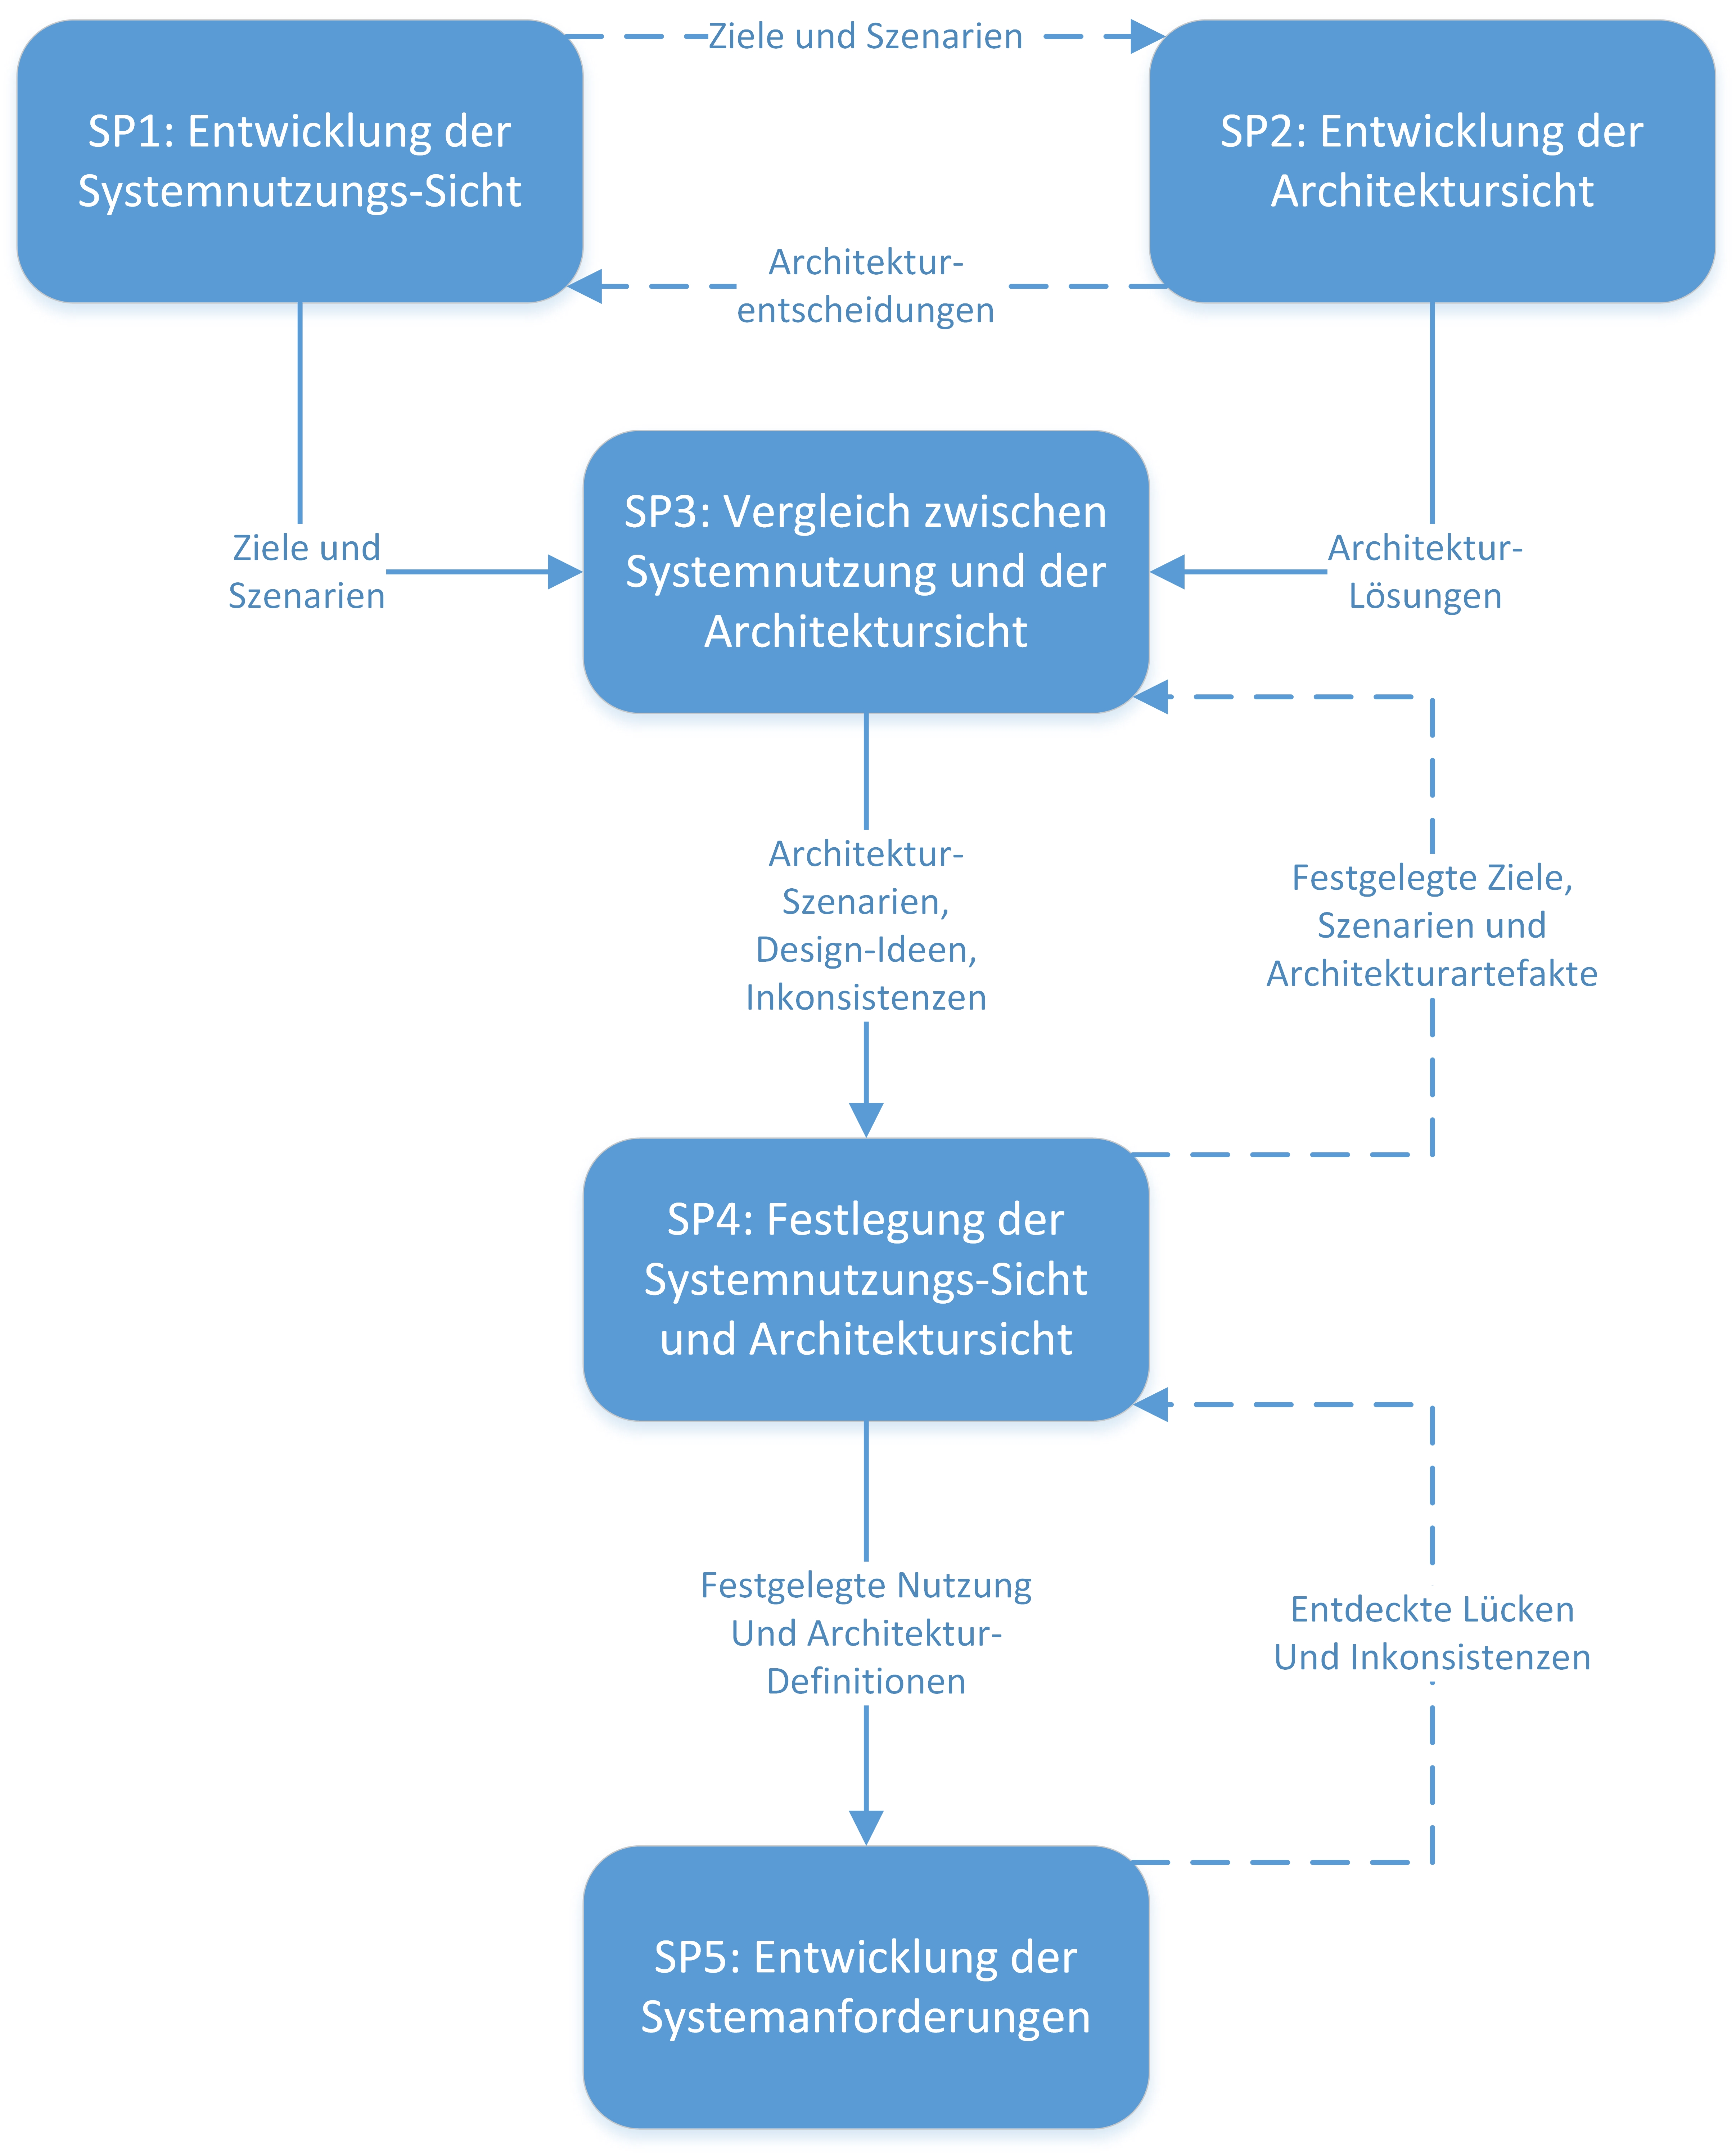
\includegraphics[scale=0.65]{COSMODRE5prozesse.jpg} 
	\caption{Die fünf Subprozesse der COSMOD-RE Methode}\label{fig:pro5}
\end{figure}

Im Rahmen der fünf Subprozesse werden folgende Artefakte generiert:\\

\begin{itemize}
\item Kontextmodell:\\
Das Kontextmodell dokumentiert die beabsichtigte Einbettung des Systems in seine Systemumgebung. Es werden externe Akteure definiert, die mit dem System interagieren. Ein Akteur kann hierbei ein Mensch oder ein System sein. Ferner wird modelliert, wie Akteure mit dem System interagieren.
\item Systemnutzungs-Ziele:\\

\item Systeminteraktions-Szenarien:
\item Architektur-Szenarien:
\item Grobe System-Architektur:
\item Systemanforderungen:
\end{itemize}

\paragraph{Entwicklung der Systemnutzungs-Sicht}
text\\

\paragraph{Entwicklung der Architektursicht}
text\\

\paragraph{Vergleich zwischen Systemnutzungs-Sicht und Architektursicht}
text\\

\paragraph{Entwicklung der Systemanforderungen}
text\\

---TODO--- Vorgehensmodell beschreiben\\

\begin{itemize}
\item[1] System: Die Systemebene beschreibt die oberste Ebene, bei der in der Anforderungssicht das System als ganzes betrachtet wird. Im Fokus stehen dabei die Interaktionen mit dem System. Weiter werden funktionale Anforderungen und Qualitätsanforderungen erstellt, die sich auf das Gesamtsystem beziehen. Die Architektursicht konzentriert sich hier auf die Definition von externen Systemschnittstellen. Hier definierte Artefakte sollen primär die Kommunikation mit Stakeholdern unterstützen.
\item[2] Komponenten: Die Komponentenebene bezeichnet die Aufteilung des Systems in einzelne Komponenten aus denen sich dieses zusammensetzen soll. Für jede Komponente werden funktionale Anforderungen und Qualitätsanforderungen formuliert. Da in dieser Ebene die Basis für die Systemarchtitektur gelegt wird, hat die Kommunikation zwischen dem Software-Architekten und dem Requirements Engineer von besonderer Bedeutung. 
\item[3] Hard-/Software Komponenten: Auf dieser Ebene werden die zuvor erstellten Komponenten in Hard- und Software Komponenten aufgeteilt und weiter verfeinert. Anforderungen auf dieser Ebene sind somit speziell auf die Komponentenart bezogen. 
\item[4] Deployment: Auf dieser Ebene werden Softwarekomponenten programmierbaren Hardwarekomponeten zugeordnet. Anforderungen auf dieser Ebene beziehen sich auf das Deployment der Softwarekomponenten und ihrem Einfluss auf vorher definierte Anforderungen. 
\end{itemize}
Da die Zusammenarbeit zwischen Software-Architekt und Requirements Engineer vor allem in den obersten beiden Ebenen von Relevanz ist, sind die unteren beiden Ebenen in diesem Kontext zu vernachlässigen.\\

Im Rahmen der Erstellung der Software-Architektur und der Anforderungen gibt es drei Co-Design Prozesse die sich wiederum in fünf Sub-Prozesse unterteilen lassen. Bei Ausführung der Prozesse werden als Artefakte sowohl die System-Architektur als auch Ziele, Szenarien und Anforderungen erzeugt. \\

\paragraph{Ausgabe}
Ausgabe der Methode ist eine kompakte Menge von System-Nutzung-Zielen, System-Interaktions-Szenarien und grobe Architekturartefakte. Ferner wird eine detaillierte System-Anforderungsspezifikation generiert.\\


\subsection{Alter Teil}
Bla\\

\subsubsection{Beschreibung}
In der Anforderungserhebung soll es m\"oglich sein Anforderungen in einer Form zu erheben, die es Software Architekten einfacher macht, den Architekturentwurf zu konzipieren. Um dies zu realisieren bietet sich eine Kombination aus Ziel-basierten Ans\"atzen und Szenario-basierten Ans\"atzen an. Die Kombination ist deswegen von Relevanz, weil ein Ansatz allein nicht ausreichen kann um die Anforderungen in angemessener Weise zu erheben.\\

\subsubsection{Ziel-basierte Ans\"atze}
Ziel-basierte Ans\"atze zielen vorrangig darauf ab, ein umfassendes Verst\"andnis der W\"unsche und Ziele der Stakeholder sowie auf die zu erzielenden Auswirkungen auf die Systemumgebung ab (Silkora Referenz S.18). Dies bedeutet, dass es bei Ziel-basierten Ans\"atzen vor allem darauf ankommt, zu verstehen, welche Vision der Stakeholder von dem Zuk\"unftigen System hat. Bei der Erfassung dieser Vision ist ein nat\"urlichsprachlicher Ansatz fehlerbehaftet, da hier sehr aufw\"andige manuelle Konsistenzpr\"ufungen notwendig w\"aren. Deswegen bieten sich hier vor allem Modell-basierte Ans\"atze an.\\

Ein gutes Beispiel f\"ur ein Modell-basierten Ansatz ist der KAOS-Ansatz. Dieser Ansatz bietet den Vorteil, dass er mit wenigen pr\"azise formulierten Modellierungsobjekten auskommt. Dies ist deswegen ein Vorteil, weil so kein besonders tief reichendes Fachwissen notwendig ist um das Modell zu interpretieren. Ferner ist der Ansatz f\"ur die Konzeption softwareintensiver eingebetteter Systeme geeignet, was eine verzahnte Entwicklung von Anforderungen und Architektur \"uber mehrere Abstraktionsstufen hinweg erm\"oglicht (Silkora Referenz S.31).\\

\paragraph{KAOS}
Lamsweerde (Lamsweerde Referenz) beschreibt eine modellbasierten Ansatz zur Darstellung von Zielen und den Referenzen innerhalb von Zielen. Hierf\"ur muss zun\"achst eine genauere Betrachtung der Zieldefinition vorgenommen werden. So sind in dem Kontext der KAOS-Methode Ziele in Bahavioral-Goals und Soft-Goals zu unterteilen. \\

Behavioral-Goals beschreiben eine deklarative Sicht auf Ziele, die beschreibt, wie ein System sich zu verhalten hat. Dies bedeutet, dass in diesem Fall besonders das Verhalten von Systemen im Fokus steht. G\"ultig ist eine endliche Menge von Verhaltensweisen des Systems. \\

Grunds\"atzlich lassen sich Bahavioral-Goals in zwei Kategorien aufteilen, die Achive-Goals und die Maintain/Avoid-Goals. Die Achive-Goals beschreiben Systemverhalten, bei dem es darauf ankommt, dass ein System zu einem definierten Zeitpunkt einen definierten Zustand erreicht. Maintain/Avoid-Goals beschreiben Systemverhalten, bei dem es darauf ankommt, dass ein System \"uber einen definierten Zeitraum hinweg einen definierten Zustand aufrechterh\"alt, oder einen definierten Zustand vermeidet.\\

Soft-goals beschreiben Pr\"aferenzen innerhalb von g\"ultigen Systemverhaltensweisen. Diese lassen sich zun\"achst in funktionale Ziele und nicht funktionale Ziele aufteilen. Die funktionalen Ziele k\"onnen die folgenden Kategorien haben:
\begin{itemize}
\item Satisfaction: Funtionale Ziele, die sich damit besch\"aftigen User-Anfragen zu beantworten.
\item Information: Funtionale Ziele, die damit besch\"aftigt sind User \"uber wichtige Systemzust\"ande zu informieren.
\item Stim-response: Funktionale Ziele, die sich damit besch\"aftigen auf Events eine angemessene Reaktion zu erzeugen.
\end{itemize}
Mit dem gegebenen Ziel die Zusammenarbeit zwischen Requirements Engineer und Software Architekt zu optimieren sind vor allem die funktionalen Ziele der Soft-Goals und die Behavioral-Goals von Relevanz.\\

der KAOS Ansatz, der die zuvor beschriebenen Zielarten als Grundlage nutzt, verwendet zur Modellierung Und-/Oder-Graphen, die in diesem Kontext Zieldiagramm genannt werden. Jedes im Graphen modellierte Ziel wird zun\"achst durch eine Reihe von Eigenschaften in einer Zielschablone charakterisiert. Die Eigenschaften k\"onnen unter anderem Name, Definition, Quelle, Zielkategorie und Priorit\"at sein.\\

--TODO-- Erzeugung Abbildung Und-Oder-Graph + Beschreibung der Elemente\\

Das Problem von Ziel-basierten Ans\"atzen wie dem KAOS Ansatz ist, dass eine Software Architektur allein basierend auf den Zielen wichtige Aspekte vernachl\"assigt. So zum Beispiel welche Rolle diese Ziele erreichen soll und gegebenenfalls wie die dieses Ziel umzusetzen ist. Daher ist es notwendig Szenario-basierte Ans\"atze zu betrachten.\\

\subsubsection{Szenario-basierte Ans\"atze}
Szenario-basierte Ans\"atze zielen vorrangig darauf ab, die wesentlichen geforderten Interaktionen des Systems mit dessen Umgebung zu definieren und mit den Stakeholdern abzustimmen (Silkora Referenz S.18).\\

Um die optimale Zusammenarbeit zu st\"utzen ist es notwendig, die Szenarien in einer Kombination aus Anwendungsfalldiagrammen und Message Sequence Charts graphisch zu modellieren. Dadurch, kann der Zusammenhang zwischen Szenarien aufgezeigt werden und wichtige Aspekte, die von Bedeutung f\"ur den Design der Softwarearchitektur sind, ber\"ucksichtigt werden. Es ist mit diesem Vorgehen m\"oglich Szenarien zu komplexeren Szenarien zusammenzusetzen und des weiteren Iterationen und alternative Szenarienverl\"aufe abzubilden (Silkora Referenz S.33). Bei der Betrachtung von Szenarien ist es jedoch auch hier notwendig, diese zun\"achst in Schablonen zu dokumentieren, um eine pr\"azise Beschreibung zu haben. In einer Schablone soll unter anderem festgehalten werden, welche prim\"aren und sekund\"aren Akteure gegeben sind. Ferner sollen eine Kurzbeschreibung und mit dem Szenario verkn\"upfte Ziele gegeben sein, um klar hervorzuheben, in welchem Kontext das Szenario zu sehen ist.\\

\paragraph{Anwendungsfalldiagramm}
Das Anwendungsfalldiagramm zeigt eine \"Ubersicht \"uber die Anwendungsf\"alle eines Systems oder einer Systemkomponente. Es stellt zudem die Akteure des Systems (der Komponente) und deren Beteiligung an den Anwendungsf\"allen grafisch dar (Silkora Zitat S.34). \\

Anwendungsf\"alle k\"onnen als Oberbegriff f\"ur Szenarien betrachtet werden, da ein Szenario sich aus einem Anwendungsfall generieren l\"asst. Dies bedeutet ein Anwendungsfall kann Grundlage für eine Vielzahl von Szenarien sein. \\

--TODO-- Anwendungsfalldiagramm beispielabbildung mit Notationselementen\\

Zu den Notationselementen eines Anwendungsfalldiagramms z\"ahlen:
\begin{itemize}
\item Akteur: Als Akteur l\"asst sich eine Person oder Entit\"at bezeichnen, die mit dem zu konzipierenden System in Beziehung steht. Diese k\"onnen zum Beispiel Nutzer sein, die \"uber eine Eingabemaske Daten eintragen sollen.
\item Systemgrenze: Systemgrenzen umschlie\ss{}en das geplante System. Akteure, die mit dem System interagieren befinden sich au\ss{}erhalb der Systemgrenze, w\"ahrend die dem System zugeordneten Anwendungsf\"alle sich innerhalb der Systemgrenze befinden.
\item Anwendungsfall: Ein Anwendungsfall beschreibt eine Funktionalit\"at des geplanten Systems. In Kombination mit dem Akteur, der in Relation zu einem Anwendungsfall steht, wird dargestellt, was das System machen soll.
\item Erweiterung eines Anwendungsfalls: Ein Anwendungsfall kann mittels Include- oder Extend-Beziehung erweitert werden. Dies soll es erm\"oglichen komplexere Anwendungsf\"alle abzubilden und gleichzeitig die Anzahl der Redundanzen m\"oglichst gering halten. Eine Include-Beziehung bedeutet hierbei, dass ein Anwendungsfall einen weiteren Anwendungsfall beinhaltet. Die Extend-Beziehung bedeutet, dass es zu einem Anwendungsfall eine Erweiterung unter einer Bedingung gibt. Die Bedingung gibt an welche Konditionen erfüllt sein müssen dass die Erweiterung greift.
\end{itemize}
Anwendungsfalldiagramme stellen Akteure und Anwendungsfälle dar. Dadurch wird veranschaulicht welche Akteure mit welchen Anwendungsfällen in Beziehung stehen und ob es wichtige Beziehungen zwischen verschiedenen Anwendungsfällen gibt. Grundsätzlich ist es möglich Anwendungsfalldiagramme auf verschiedenen Abstraktionsstufen abzubilden um so sowohl für das Gesamtsystem, als auch für die Teilsysteme die Beziehungen zu betrachten. Um jedoch Szenarien präzise zu spezifizieren reichen Anwendungsfalldiagramme nicht aus.\\

\paragraph{Message-Sequence-Charts}
Mithilfe von Message-Sequence-Charts ist es möglich eine präzise Spezifikation der verschiedenen Szenarien eines Anwendungsfalls zu generieren (Silkora Zitat S.37). Bei der Betrachtung der Zusammenarbeit zwischen Software-Architekt und Requirements-Engineer ist zunächst nur eine Teilmenge der Notationselemente der Message-Sequence-Charts relevant. Wichtigster Aspekt der Message-Sequence-Charts ist, dass diese vor allem die Akteure und ihre Interaktionen mit dem System hervorheben.\\

Grundsätzlich werde in einem Message-Sequence-Chart Nachrichten und Instanzen abgebildet. Eine Instanz kann hierbei z.B. ein System oder ein Akteur sein. Als Nachricht wird im Kontext der Message-Sequence-Charts der Austausch einer Information bezeichnet. Dies können z.B. Signale oder Daten sein, die zwischen den Instanzen versendet werden (Silkora Referenz S.38). \\

--TODO-- Abbildung zu MSC und Beschreibung\\

Neben den einfachen Message-Sequence-Charts gibt es High-Level-Message-Sequence-Charts (HLMSC), die es ermöglichen eine Komposition mehrerer Message-Sequence-Charts zu bilden und so komplexere Zusammenhänge darzustellen. Grundsätzlich besteht ein HLMSC aus einem Start- und Endknoten, einem oder mehreren Verweisknoten und einer Menge von Kanten. Die Start- und Endknoten dienen hierbei der Begrenzung des Anwendungsfalls.  Die Verweisknoten sind als Verweise zu einfachen Message-Sequence-Charts oder weiteren HLMSC zu sehen. Ungerichtete Kanten dienen der Darstellung der Komposition und mithilfe von gerichteten Kanten lässt sich Iteration darstellen.\\

--TODO-- Abbildung zu HLMSC \\

Wenn Anwendungsfälle in Kompositionen zusammengefasst werden lässt sich argumentieren, dass man bei hinreichenden Kompositionen in den Bereich der Ziele gelangt. Somit wird deutlich, dass der Szenario-basierte Ansatze implizit schon eine Betrachtung der Ziele fordert.\\

\subsubsection{Kombination der Ans\"atze}
Wenn die wesentlichen Ziele der Stakeholder bekannt sind, besteht die M\"oglichkeit, diejenige Architekturalternative auszuw\"ahlen, mit der die Ziele am besten erf\"ullt werden k\"onnen (Silkora Referenz S.18).\\

Sowohl Ziel-basierte Ansätze als auch Szenario-basierte Ansätze sind alleinstehend nicht ausreichend, um eine Grundlage für einen guten Architekturansatz auf der Basis von Anforderungen zu generieren. Hierfür ist es notwendig, die Ansätze zu kombinieren. \\

Ein Beispiel für eine solche Kombination ist der COSMOD-RE (sCenario and gOal based SysteM develOpment methoD) Ansatz. \\

\paragraph{COSMOD-RE}



--TODO-- Abbildung Zu den Sub-prozessen des Designs\\

\subsubsection{Bewertung}
In der Betrachtung Ziel-basierter Ansätze wird deutlich, dass diese allein nicht ausreichen um weitreichende Architekturentscheidungen zu treffen. Hauptproblem ist hier, dass mithilfe der Ziele lediglich angegeben wird, was am Ende aus der Sicht der Stakeholder erreicht werden soll und nicht konkret welche Rolle in dem System welche Aufgaben hat und wie das Ziel zu erreichen ist.\\

Szenario-basierte Ansätze deuten an, dass diese alleinstehend ebenfalls nicht ausreichen um eine Software-Architektur zu entwerfen, da hier vor allem das Problem besteht, dass alleinstehende Szenarien ohne Zusammenhang am Ende der Entwicklung keine konsistentes System ergeben können. Durch Ziele werden sie in den richtigen Kontext gesetzt, was bei Szenario-basierten Ansätzen die Formulierung von Zielen voraussetzt.\\

Gemeinsame Ansätze wie der COSMOD-RE Ansatz verbinden Szenario- und Ziel-basierte Ansätze und ermöglichen es so mithilfe eines Iterativen Vorgehens die Grundlage für ein Architekturentwurf zu generieren, dass sowohl die Wünsche des Kunden widerspiegelt als auch ausführlich genug ist.
